\documentclass[tikz,border=5pt]{standalone}
\usepackage[T1]{fontenc}
\usepackage{lmodern,amsmath,amssymb}
\usetikzlibrary{arrows.meta,calc,positioning,fit,backgrounds,shapes.geometric,matrix,decorations.pathreplacing,patterns}
\definecolor{ink}{gray}{0.08}
\definecolor{wash}{gray}{0.965}
\definecolor{soft}{gray}{0.45}
\tikzset{box/.style={draw=ink,line width=.65pt,fill=white,align=center,inner sep=4pt,outer sep=0pt,font=\small},flow/.style={draw=ink,line width=.65pt,-{Latex[length=1.8mm,width=1.3mm]},rounded corners=2pt},annotation/.style={font=\scriptsize,text=soft,align=center},groupbox/.style={draw=soft,dashed,line width=.45pt,fill=wash}}
\begin{document}
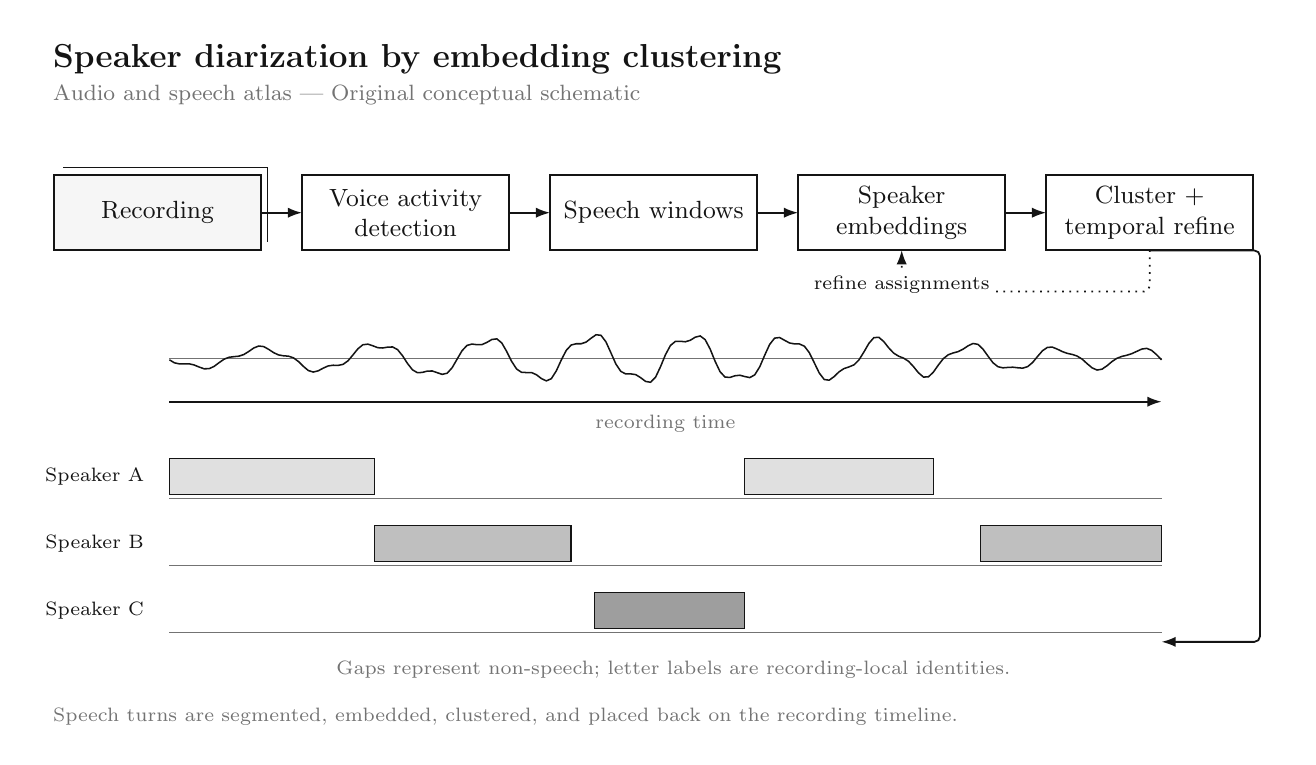
\begin{tikzpicture}[x=1cm,y=-1cm,font=\rmfamily,text=ink]

\path[use as bounding box] (0,0) rectangle (16,9);
\node[anchor=west,font=\large\bfseries] at (.2,.4) {Speaker diarization by embedding clustering};
\node[anchor=west,font=\footnotesize,text=soft] at (.2,.85) {Audio and speech atlas | Original conceptual schematic};
\begin{pgfonlayer}{background}
\end{pgfonlayer}
\node[box,fill=wash,minimum width=2.6cm,minimum height=0.95cm,text width=2.35cm] (audio) at (1.65,2.35) {Recording};
\draw[ink,line width=.4pt] (0.44999999999999984,1.775) -- (3.0500000000000003,1.775) -- (3.0500000000000003,2.725);
\node[box,minimum width=2.6cm,minimum height=0.95cm,text width=2.35cm] (vad) at (4.8,2.35) {Voice activity\\detection};
\node[box,minimum width=2.6cm,minimum height=0.95cm,text width=2.35cm] (seg) at (7.95,2.35) {Speech windows};
\node[box,minimum width=2.6cm,minimum height=0.95cm,text width=2.35cm] (emb) at (11.1,2.35) {Speaker\\embeddings};
\node[box,minimum width=2.6cm,minimum height=0.95cm,text width=2.35cm] (cluster) at (14.25,2.35) {Cluster +\\temporal refine};
\begin{pgfonlayer}{background}
\draw[flow] (audio.east) -- (vad.west);
\draw[flow] (vad.east) -- (seg.west);
\draw[flow] (seg.east) -- (emb.west);
\draw[flow] (emb.east) -- (cluster.west);
\draw[flow,dotted] (cluster.south) -- (14.25,3.35) -- (11.1,3.35) -- (emb.south) node[midway,below,fill=white,inner sep=1.5pt,font=\scriptsize] {refine assignments};
\end{pgfonlayer}
\draw[soft,line width=.35pt] (1.8,4.2) -- (14.4,4.2);
\draw[ink,line width=.55pt] plot coordinates {(1.800,4.218) (1.863,4.256) (1.926,4.270) (1.989,4.269) (2.052,4.269) (2.115,4.284) (2.178,4.310) (2.241,4.332) (2.304,4.331) (2.367,4.302) (2.430,4.255) (2.493,4.211) (2.556,4.186) (2.619,4.178) (2.682,4.172) (2.745,4.151) (2.808,4.112) (2.871,4.068) (2.934,4.043) (2.997,4.050) (3.060,4.085) (3.123,4.127) (3.186,4.156) (3.249,4.167) (3.312,4.172) (3.375,4.193) (3.438,4.239) (3.501,4.301) (3.564,4.354) (3.627,4.374) (3.690,4.358) (3.753,4.324) (3.816,4.296) (3.879,4.287) (3.942,4.289) (4.005,4.276) (4.068,4.231) (4.131,4.156) (4.194,4.078) (4.257,4.027) (4.320,4.019) (4.383,4.040) (4.446,4.064) (4.509,4.068) (4.572,4.057) (4.635,4.055) (4.698,4.089) (4.761,4.167) (4.824,4.265) (4.887,4.345) (4.950,4.382) (5.013,4.378) (5.076,4.361) (5.139,4.360) (5.202,4.382) (5.265,4.403) (5.328,4.388) (5.391,4.318) (5.454,4.209) (5.517,4.102) (5.580,4.035) (5.643,4.018) (5.706,4.026) (5.769,4.025) (5.832,3.997) (5.895,3.960) (5.958,3.952) (6.021,4.004) (6.084,4.113) (6.147,4.239) (6.210,4.336) (6.273,4.377) (6.336,4.380) (6.399,4.380) (6.462,4.408) (6.525,4.457) (6.588,4.486) (6.651,4.457) (6.714,4.358) (6.777,4.220) (6.840,4.098) (6.903,4.030) (6.966,4.014) (7.029,4.014) (7.092,3.993) (7.155,3.944) (7.218,3.900) (7.281,3.907) (7.344,3.990) (7.407,4.129) (7.470,4.271) (7.533,4.365) (7.596,4.398) (7.659,4.397) (7.722,4.406) (7.785,4.445) (7.848,4.493) (7.911,4.503) (7.974,4.439) (8.037,4.306) (8.100,4.153) (8.163,4.036) (8.226,3.984) (8.289,3.983) (8.352,3.989) (8.415,3.970) (8.478,3.931) (8.541,3.915) (8.604,3.962) (8.667,4.081) (8.730,4.236) (8.793,4.369) (8.856,4.437) (8.919,4.442) (8.982,4.421) (9.045,4.414) (9.108,4.431) (9.171,4.444) (9.234,4.409) (9.297,4.307) (9.360,4.160) (9.423,4.023) (9.486,3.943) (9.549,3.935) (9.612,3.970) (9.675,4.004) (9.738,4.016) (9.801,4.017) (9.864,4.045) (9.927,4.128) (9.990,4.256) (10.053,4.386) (10.116,4.468) (10.179,4.477) (10.242,4.431) (10.305,4.370) (10.368,4.329) (10.431,4.308) (10.494,4.282) (10.557,4.220) (10.620,4.119) (10.683,4.010) (10.746,3.937) (10.809,3.932) (10.872,3.986) (10.935,4.066) (10.998,4.133) (11.061,4.172) (11.124,4.197) (11.187,4.237) (11.250,4.305) (11.313,4.383) (11.376,4.437) (11.439,4.435) (11.502,4.375) (11.565,4.285) (11.628,4.204) (11.691,4.154) (11.754,4.131) (11.817,4.114) (11.880,4.082) (11.943,4.040) (12.006,4.011) (12.069,4.022) (12.132,4.082) (12.195,4.170) (12.258,4.254) (12.321,4.305) (12.384,4.320) (12.447,4.315) (12.510,4.312) (12.573,4.319) (12.636,4.324) (12.699,4.305) (12.762,4.253) (12.825,4.176) (12.888,4.103) (12.951,4.060) (13.014,4.057) (13.077,4.083) (13.140,4.114) (13.203,4.136) (13.266,4.150) (13.329,4.171) (13.392,4.210) (13.455,4.267) (13.518,4.320) (13.581,4.348) (13.644,4.337) (13.707,4.294) (13.770,4.241) (13.833,4.199) (13.896,4.175) (13.959,4.160) (14.022,4.140) (14.085,4.111) (14.148,4.082) (14.211,4.073) (14.274,4.098) (14.337,4.153) (14.400,4.218)};
\draw[flow] (1.8,4.75) -- (14.4,4.75);
\node[align=center,anchor=center,font=\scriptsize,text=soft,text width=3cm] at (8.1,5.03) {recording time};
\node[align=center,anchor=center,font=\scriptsize,text=ink,text width=1.6cm] at (0.85,5.7) {Speaker A};
\draw[soft,line width=.3pt] (1.8,5.98) -- (14.4,5.98);
\draw[ink,fill=black!12] (1.8,5.47) rectangle (4.4,5.930000000000001);
\draw[ink,fill=black!12] (9.1,5.47) rectangle (11.5,5.930000000000001);
\node[align=center,anchor=center,font=\scriptsize,text=ink,text width=1.6cm] at (0.85,6.55) {Speaker B};
\draw[soft,line width=.3pt] (1.8,6.83) -- (14.4,6.83);
\draw[ink,fill=black!25] (4.4,6.319999999999999) rectangle (6.9,6.78);
\draw[ink,fill=black!25] (12.1,6.319999999999999) rectangle (14.4,6.78);
\node[align=center,anchor=center,font=\scriptsize,text=ink,text width=1.6cm] at (0.85,7.4) {Speaker C};
\draw[soft,line width=.3pt] (1.8,7.680000000000001) -- (14.4,7.680000000000001);
\draw[ink,fill=black!38] (7.2,7.17) rectangle (9.1,7.630000000000001);
\draw[flow] (14.25,2.83) -- (15.65,2.83) -- (15.65,7.8) -- (14.4,7.8);
\node[align=center,anchor=center,font=\scriptsize,text=soft,text width=13cm] at (8.2,8.15) {Gaps represent non-speech; letter labels are recording-local identities.};
\node[anchor=west,align=left,font=\scriptsize,text=soft,text width=15.6cm] at (.2,8.75) {Speech turns are segmented, embedded, clustered, and placed back on the recording timeline.};
\end{tikzpicture}
\end{document}
